\documentclass{standalone}
\usepackage{tikz}
\usetikzlibrary{patterns, positioning}


\begin{document}
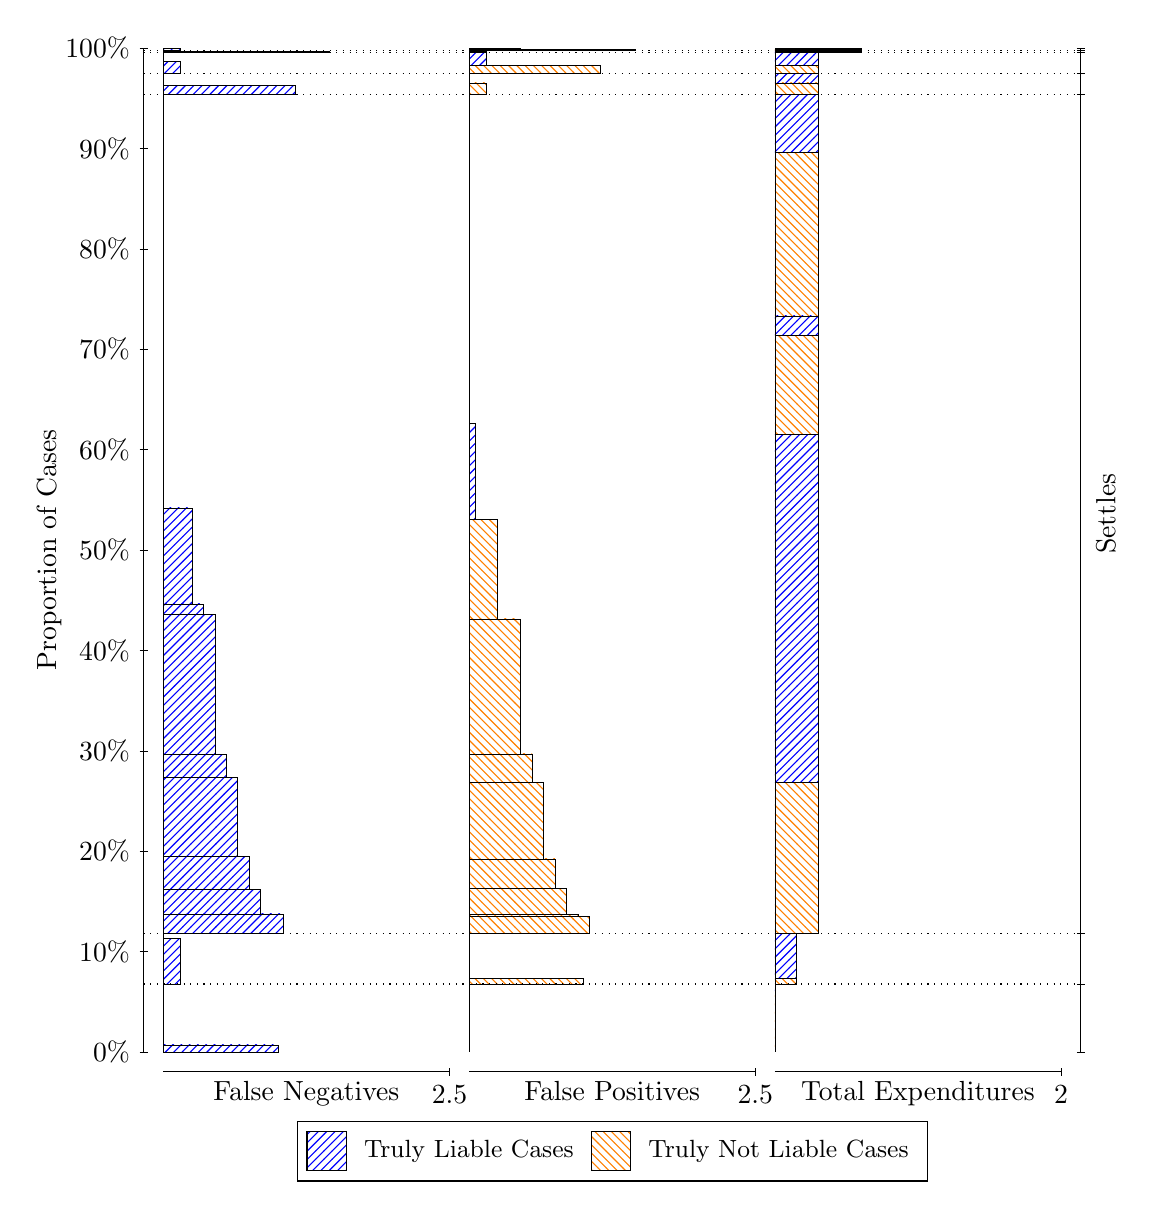
\begin{tikzpicture}
\draw[black, very thin] (1.5,1.75) -- (1.5,14.5);
\node[rotate=90, text=black, anchor=center] at (0.3, 8.125) {Proportion of Cases};
\draw[black, very thin] (1.45,1.75) -- (1.55,1.75);
\node[text=black, anchor=east] at (1.45, 1.75) {0\%};
\draw[black, very thin] (1.45,3.025) -- (1.55,3.025);
\node[text=black, anchor=east] at (1.45, 3.025) {10\%};
\draw[black, very thin] (1.45,4.3) -- (1.55,4.3);
\node[text=black, anchor=east] at (1.45, 4.3) {20\%};
\draw[black, very thin] (1.45,5.575) -- (1.55,5.575);
\node[text=black, anchor=east] at (1.45, 5.575) {30\%};
\draw[black, very thin] (1.45,6.85) -- (1.55,6.85);
\node[text=black, anchor=east] at (1.45, 6.85) {40\%};
\draw[black, very thin] (1.45,8.125) -- (1.55,8.125);
\node[text=black, anchor=east] at (1.45, 8.125) {50\%};
\draw[black, very thin] (1.45,9.4) -- (1.55,9.4);
\node[text=black, anchor=east] at (1.45, 9.4) {60\%};
\draw[black, very thin] (1.45,10.675) -- (1.55,10.675);
\node[text=black, anchor=east] at (1.45, 10.675) {70\%};
\draw[black, very thin] (1.45,11.95) -- (1.55,11.95);
\node[text=black, anchor=east] at (1.45, 11.95) {80\%};
\draw[black, very thin] (1.45,13.225) -- (1.55,13.225);
\node[text=black, anchor=east] at (1.45, 13.225) {90\%};
\draw[black, very thin] (1.45,14.5) -- (1.55,14.5);
\node[text=black, anchor=east] at (1.45, 14.5) {100\%};

\draw[black, very thin] (13.4,1.75) -- (13.4,14.5);
\draw[black, very thin] (13.35,1.75) -- (13.45,1.75);
\node[anchor=west] at (13.35, 1.75) {};
\draw[black, very thin] (13.35,2.6127) -- (13.45,2.6127);
\node[anchor=west] at (13.35, 2.6127) {};
\draw[black, very thin] (13.35,3.2597) -- (13.45,3.2597);
\node[anchor=west] at (13.35, 3.2597) {};
\draw[black, very thin] (13.35,13.912) -- (13.45,13.912);
\node[anchor=west] at (13.35, 13.912) {};
\draw[black, very thin] (13.35,14.173) -- (13.45,14.173);
\node[anchor=west] at (13.35, 14.173) {};
\draw[black, very thin] (13.35,14.444) -- (13.45,14.444);
\node[anchor=west] at (13.35, 14.444) {};
\draw[black, very thin] (13.35,14.471) -- (13.45,14.471);
\node[anchor=west] at (13.35, 14.471) {};
\draw[black, very thin] (13.35,14.5) -- (13.45,14.5);
\node[anchor=west] at (13.35, 14.5) {};

\draw[black, very thin, pattern color=blue, pattern=north east lines] (1.75,1.75) rectangle (3.2033,1.8408);
\draw[black, very thin, pattern color=orange, pattern=north west lines] (1.75,1.8408) rectangle (1.75,2.6127);
\draw[black, very thin, pattern color=blue, pattern=north east lines] (1.75,2.6127) rectangle (1.968,3.1916);
\draw[black, very thin, pattern color=orange, pattern=north west lines] (1.75,3.1916) rectangle (1.75,3.2597);
\draw[black, very thin, pattern color=blue, pattern=north east lines] (1.75,3.2597) rectangle (3.276,3.5027);
\draw[black, very thin, pattern color=blue, pattern=north east lines] (1.75,3.5027) rectangle (2.9853,3.8116);
\draw[black, very thin, pattern color=blue, pattern=north east lines] (1.75,3.8116) rectangle (2.84,4.2358);
\draw[black, very thin, pattern color=blue, pattern=north east lines] (1.75,4.2358) rectangle (2.6947,5.2354);
\draw[black, very thin, pattern color=blue, pattern=north east lines] (1.75,5.2354) rectangle (2.5493,5.5317);
\draw[black, very thin, pattern color=blue, pattern=north east lines] (1.75,5.5317) rectangle (2.404,7.3048);
\draw[black, very thin, pattern color=blue, pattern=north east lines] (1.75,7.3048) rectangle (2.2587,7.442);
\draw[black, very thin, pattern color=blue, pattern=north east lines] (1.75,7.442) rectangle (2.1133,8.6606);
\draw[black, very thin, pattern color=orange, pattern=north west lines] (1.75,8.6606) rectangle (1.75,13.912);
\draw[black, very thin, pattern color=blue, pattern=north east lines] (1.75,13.912) rectangle (3.4213,14.027);
\draw[black, very thin, pattern color=orange, pattern=north west lines] (1.75,14.027) rectangle (1.75,14.173);
\draw[black, very thin, pattern color=blue, pattern=north east lines] (1.75,14.173) rectangle (1.968,14.333);
\draw[black, very thin, pattern color=orange, pattern=north west lines] (1.75,14.333) rectangle (1.75,14.444);
\draw[black, very thin, pattern color=blue, pattern=north east lines] (1.75,14.444) rectangle (3.8573,14.453);
\draw[black, very thin, pattern color=orange, pattern=north west lines] (1.75,14.453) rectangle (1.75,14.471);
\draw[black, very thin, pattern color=blue, pattern=north east lines] (1.75,14.471) rectangle (1.968,14.491);
\draw[black, very thin, pattern color=orange, pattern=north west lines] (1.75,14.491) rectangle (1.75,14.5);
\draw[black, very thin, pattern color=orange, pattern=north west lines] (5.6333,1.75) rectangle (5.6333,2.5219);
\draw[black, very thin, pattern color=blue, pattern=north east lines] (5.6333,2.5219) rectangle (5.6333,2.6127);
\draw[black, very thin, pattern color=orange, pattern=north west lines] (5.6333,2.6127) rectangle (7.0867,2.6808);
\draw[black, very thin, pattern color=blue, pattern=north east lines] (5.6333,2.6808) rectangle (5.6333,3.2597);
\draw[black, very thin, pattern color=orange, pattern=north west lines] (5.6333,3.2597) rectangle (7.1593,3.4722);
\draw[black, very thin, pattern color=orange, pattern=north west lines] (5.6333,3.4722) rectangle (7.014,3.494);
\draw[black, very thin, pattern color=orange, pattern=north west lines] (5.6333,3.494) rectangle (6.8687,3.8251);
\draw[black, very thin, pattern color=orange, pattern=north west lines] (5.6333,3.8251) rectangle (6.7233,4.2011);
\draw[black, very thin, pattern color=orange, pattern=north west lines] (5.6333,4.2011) rectangle (6.578,5.1702);
\draw[black, very thin, pattern color=orange, pattern=north west lines] (5.6333,5.1702) rectangle (6.4327,5.535);
\draw[black, very thin, pattern color=orange, pattern=north west lines] (5.6333,5.535) rectangle (6.2873,7.2511);
\draw[black, very thin, pattern color=orange, pattern=north west lines] (5.6333,7.2511) rectangle (5.9967,8.5113);
\draw[black, very thin, pattern color=blue, pattern=north east lines] (5.6333,8.5113) rectangle (5.706,9.7298);
\draw[black, very thin, pattern color=blue, pattern=north east lines] (5.6333,9.7298) rectangle (5.6333,13.912);
\draw[black, very thin, pattern color=orange, pattern=north west lines] (5.6333,13.912) rectangle (5.8513,14.058);
\draw[black, very thin, pattern color=blue, pattern=north east lines] (5.6333,14.058) rectangle (5.6333,14.173);
\draw[black, very thin, pattern color=orange, pattern=north west lines] (5.6333,14.173) rectangle (7.3047,14.283);
\draw[black, very thin, pattern color=blue, pattern=north east lines] (5.6333,14.283) rectangle (5.8513,14.444);
\draw[black, very thin, pattern color=orange, pattern=north west lines] (5.6333,14.444) rectangle (5.8513,14.462);
\draw[black, very thin, pattern color=blue, pattern=north east lines] (5.6333,14.462) rectangle (5.6333,14.471);
\draw[black, very thin, pattern color=orange, pattern=north west lines] (5.6333,14.471) rectangle (7.7407,14.48);
\draw[black, very thin, pattern color=blue, pattern=north east lines] (5.6333,14.48) rectangle (6.2873,14.5);
\draw[black, very thin, pattern color=orange, pattern=north west lines] (9.5167,1.75) rectangle (9.5167,2.5219);
\draw[black, very thin, pattern color=blue, pattern=north east lines] (9.5167,2.5219) rectangle (9.5167,2.6127);
\draw[black, very thin, pattern color=orange, pattern=north west lines] (9.5167,2.6127) rectangle (9.7892,2.6808);
\draw[black, very thin, pattern color=blue, pattern=north east lines] (9.5167,2.6808) rectangle (9.7892,3.2597);
\draw[black, very thin, pattern color=orange, pattern=north west lines] (9.5167,3.2597) rectangle (10.062,5.1702);
\draw[black, very thin, pattern color=blue, pattern=north east lines] (9.5167,5.1702) rectangle (10.062,9.595);
\draw[black, very thin, pattern color=orange, pattern=north west lines] (9.5167,9.595) rectangle (10.062,10.855);
\draw[black, very thin, pattern color=blue, pattern=north east lines] (9.5167,10.855) rectangle (10.062,11.098);
\draw[black, very thin, pattern color=orange, pattern=north west lines] (9.5167,11.098) rectangle (10.062,13.179);
\draw[black, very thin, pattern color=blue, pattern=north east lines] (9.5167,13.179) rectangle (10.062,13.912);
\draw[black, very thin, pattern color=orange, pattern=north west lines] (9.5167,13.912) rectangle (10.062,14.058);
\draw[black, very thin, pattern color=blue, pattern=north east lines] (9.5167,14.058) rectangle (10.062,14.173);
\draw[black, very thin, pattern color=orange, pattern=north west lines] (9.5167,14.173) rectangle (10.062,14.283);
\draw[black, very thin, pattern color=blue, pattern=north east lines] (9.5167,14.283) rectangle (10.062,14.444);
\draw[black, very thin, pattern color=orange, pattern=north west lines] (9.5167,14.444) rectangle (10.607,14.462);
\draw[black, very thin, pattern color=blue, pattern=north east lines] (9.5167,14.462) rectangle (10.607,14.471);
\draw[black, very thin, pattern color=orange, pattern=north west lines] (9.5167,14.471) rectangle (10.607,14.48);
\draw[black, very thin, pattern color=blue, pattern=north east lines] (9.5167,14.48) rectangle (10.607,14.5);
\draw[black, dotted] (1.5,2.6127) -- (13.4,2.6127);
\draw[black, dotted] (1.5,3.2597) -- (13.4,3.2597);
\draw[black, dotted] (1.5,13.912) -- (13.4,13.912);
\draw[black, dotted] (1.5,14.173) -- (13.4,14.173);
\draw[black, dotted] (1.5,14.444) -- (13.4,14.444);
\draw[black, dotted] (1.5,14.471) -- (13.4,14.471);
\draw[black, very thin] (1.75,1.5) -- (5.3833,1.5);
\node[text=black, anchor=north] at (3.5667, 1.5) {False Negatives};
\draw[black, very thin] (5.3833,1.45) -- (5.3833,1.55);
\node[text=black, anchor=north] at (5.3833, 1.45) {2.5};

\draw[black, very thin] (5.6333,1.5) -- (9.2667,1.5);
\node[text=black, anchor=north] at (7.45, 1.5) {False Positives};
\draw[black, very thin] (9.2667,1.45) -- (9.2667,1.55);
\node[text=black, anchor=north] at (9.2667, 1.45) {2.5};

\draw[black, very thin] (9.5167,1.5) -- (13.15,1.5);
\node[text=black, anchor=north] at (11.333, 1.5) {Total Expenditures};
\draw[black, very thin] (13.15,1.45) -- (13.15,1.55);
\node[text=black, anchor=north] at (13.15, 1.45) {2};



\node[text=black, centered, rotate=90] at (13.72, 8.5859) {Settles};





\draw (7.449999999999999,1.5) node[draw=none] (baseCoordinate) {};
\begin{scope}[align=center]
        \matrix[scale=0.5, draw=black, below=0.5cm of baseCoordinate, nodes={draw}, column sep=0.1cm]{
            \node[rectangle, draw, minimum width=0.5cm, minimum height=0.5cm, pattern color=blue, pattern=north east lines] {}; &
            \node[draw=none, font=\small, text=black] (B) {Truly Liable Cases}; &
            \node[rectangle, draw, minimum width=0.5cm, minimum height=0.5cm, pattern color=orange, pattern=north west lines] {}; &
            \node[draw=none, font=\small, text=black] (B) {Truly Not Liable Cases}; \\
            };
\end{scope}

\end{tikzpicture}
\end{document}